\documentclass{article}
\usepackage{amsthm}
\usepackage{algpseudocode} 
\usepackage{graphicx}

\theoremstyle{definition}
\newtheorem{definition}{Definition}

\theoremstyle{definition}
\newtheorem{algorithm}{Algorithm}

\theoremstyle{theorem}
\newtheorem{claim}{Claim}
\newtheorem*{lemma}{Lemma}

\title{Minesweeper Solver Analysis}
\author{Jacob Slagle}


\begin{document}
	\maketitle
	
	\section*{Introduction}
	This document discusses in detail my thought process in developing the algorithms. As a disclaimer I'd like to say that I understand that writing code doesn't usually include theoretical analysis like this, and in fact I wrote this document after coding up the algorithms I've described. The reason I wrote this is to explain my thought process in developing the solver algorithms, i.e. to demonstrate how I can see the essential, theoretical nature of a problem and from there develop effective and efficient algorithms. This theoretical clarity is useful both in terms of organizing code and communicating with teammates.
	
	
	Henceforth I will mostly stick to the formal "we" is in mathematical writing.
	
	To begin with we consider the problem of beating a game of minesweeper. Simply put, we are trying to decide squares have mines and which do not. If we can find some such squares we flag the ones that have mines and reveal or "click" the squares that don't. In doing so, we have more information which helps us decide more squares to flag or reveal. As long as we can keep finding squares, eventually we'll cover the whole board and in this way we win the game.
	\section*{Human-like Solving}
	As a starting point we consider how a person plays minesweeper, as opposed to a computer executing an algorithm. Dropping the formal "we" momentarily, if I can formalize the strategies I use to play minesweeper (I'm assuming not everybody plays in exactly the way I  do), I can turn them into an algorithm.
	
	\subsection*{The Strategies}
	When I play minesweeper, my bread and butter strategy is to consider the information provided a by looking at a number on the board, or by looking at two numbers in conjunction and seeing if I can deduce where mines must be, or where mines must not be. Consider this example:
	\begin{center}
		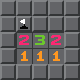
\includegraphics[width=0.2\textwidth]{exampleimages/example1a}
	\end{center}
	 There is a 3 on the board with only one flag next to it and exactly two blank squares next to it (i.e. the other five squares adjacent to it have been revealed).The 3 requires two more flags to satisfy it, and since only two blank squares adjacent to 3 remain we know those must contain mines and so we flag them
	\begin{center}
		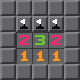
\includegraphics[width=0.2\textwidth]{exampleimages/example1b}
	\end{center}
	In doing so we are following a certain strategy: if the number of spaces around a number equals the number of flags that still need to be placed around it, then flag all those spaces. We now formalize that strategy. Let $p$ be a point on the board, and let $m$ be the number of mines around $p$ that need to be flagged beyond those that have already been flagged, and let $B$ be the blank squares adjacent to $p$ (in the above example, $m = 2$ and $|B| = 2$). We state the strategy in a pseudocode snippet:
	\begin{algorithmic}
		\If{$m = |B|$} \Comment strategy 1
		\State flagAll($B$)
		\EndIf
	\end{algorithmic}
	We also know that if there are no more flags required, then we can simply reveal all adjacent squares
	\begin{algorithmic}
		\If{$m = 0$} \Comment strategy 2
		\State revealAll($B$)
		\EndIf
	\end{algorithmic}
	
	Those are the two strategies we follow when we look at one number. Now consider this example with two numbers. 
	\begin{center}
		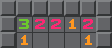
\includegraphics[width=0.3\textwidth]{exampleimages/example2a}
	\end{center}
	Consider the 2 in the center and the 1 directly to the right of it. There are two squares adjacent to both of them, the space above the 2 and above the 1. Because these squares are adjacent to the 1, only one of them can contain a mine. But the 2 must have two mines adjacent to it, and so there must be another mine elsewhere to satisfy it. Outside of these two spaces shared by the one and two, the only blank square is above and to the left of the 2, so we flag this space:
	\begin{center}
		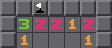
\includegraphics[width=0.3\textwidth]{exampleimages/example2b}
	\end{center}
	To capture this idea in a strategy we define some variables: Ilet $p_1$ and $p_2$ two points on the board, let $m_1$ and $m_2$ the number of mines needed to satisfy $p_1$ and $p_2$ respectively, and let $B_1$ and $B_2$ be the blank squares around $p_1$ and $p_2$ respectively. Set $I = B_1 \cap B_2$.  Observe that since $I \subseteq B_1$ it can not contain any more mines than $B_1$ which contains $m_1$ mines, that is $I$ can not contain more mines that $B_1$. We can apply the same logic with $B_2$ instead of $B_1$, and of course $I$ can not have more mines than spaces, and so altogether we have a bound on the number of mines in $I$
	$$i _{max} = \textrm{max}(m_1,m_2,|I|) $$
	With these definitions we state this strategy
	\begin{algorithmic}
		\If{$m_1 - i_{max} = |B_1 - I|$} \Comment Strategy 3
		\State flagAll($B_1 - I$)
		\EndIf
	\end{algorithmic}
	as well as the symmetric strategy
	\begin{algorithmic}
		\If{$m_2 - i_{max} = |B_2 - I|$} \Comment Strategy 4
		\State flagAll($B_2 - I$)
		\EndIf
	\end{algorithmic}
	If we call the 1 in our example $p_1$ and the 2 is $p_2$, then the strategy we used is Strategy 4. 
	
	We can also establish a \textit{lower} bound $i_{min}$ on the number of flags in $I$. Namely, $B_1 - I$ can only contain $|B_1 - I|$ mines, and so $I$ must contain the remaining $m_1 - |B_1 - I|$ mines required around $p_1$. Similarly $I$ must contain at least $m_2 - |B_2 - I|$ mines, and so we say
	$$i_{min} = \textrm{max}(m_1 - |B_1 - I|, m_2 - |B_2 - I|)$$
	Using this we derive three more strategies:
	\begin{algorithmic}
		\If{$i_{min} = |I|$} \Comment Strategy 5
		\State flagAll($I$)
		\EndIf
	\end{algorithmic}
	\begin{algorithmic}
		\If{$i_{min} = m_1$} \Comment Strategy 6
		\State revealAll($B_1 - I$)
		\EndIf
	\end{algorithmic}
	\begin{algorithmic}
		\If{$i_{min} = m_2$} \Comment Strategy 7
		\State revealAll($B_2 - I$)
		\EndIf
	\end{algorithmic}
	In fact, if we apply Strategy 6 to our example (with $p_1$ as the 1 and $p_2$ as the 2, as before), we are able to reveal a square:
	\begin{center}
		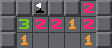
\includegraphics[width=0.3\textwidth]{exampleimages/example2c}
	\end{center}
	
	\subsection*{Human-like Algorithm }
	The basic idea for the algorithm is to just apply to the strategies to different points (or pairs of points) on the board until the game is won. It's just a matter of deciding when and where to apply the strategies. First off, observe that there is no use in applying Strategies 3-7 unless the two points have at least one blank neighbor in common. With this in mind, we write a subroutine that takes a point $p$ and applies all the necessary strategies to it.
	\begin{algorithmic}
		\Function{ApplyStrategies}{$p$}
		\State Apply Strategies 1 and 2 to $p$
		\State $p_1 \gets p$
		\ForAll{points $p_2$ that share a blank neighbor with $p_1$}
		\State Apply Strategies 3-7 to $p_1$ and $p_2$
		\EndFor
		\EndFunction
	\end{algorithmic}
	Now its just a question of which points to call ApplyStrategies on. Firstoff, we only need to check revealed points, i.e. squares with numbers. Secondly we only need to bother with points that have at least one blank neighbor- we will call the collection of all such points the \textbf{fringe} because it consists of those squares on the edge of the contiguous blobs of revealed squares. Finally, while we may meed to call ApplyStrategies repeatedly on a given point $p$, we only need to call it again \textit{after} one of the blank neighbors of $p$ has been flagged or revealed. To capture this we'll have a stack active which tracks which points need to be checked (which may have repeated values). Here is the pseudocode to solve a game $G$ of minesweeper. We assume at least one move has been made so that there are revealed squares and a fringe to begin with
		\begin{algorithmic}
		\Function{Solve}{$G$} \Comment Human-Like algorithm
		\State $active \gets$ fringe of $G$
		\While{$active$ is not empty}
		\State $p \gets active.\textrm{pop()}$
		\State ApplyStrategies($p$)
		\ForAll{revealed points $q$ with a just revealed/flagged neighbor}
		\State $active$.push($q$)
		\EndFor
		\EndWhile
		\EndFunction
	\end{algorithmic}

	
	\subsection*{Correctness and Completeness}
	The correctness of the algorithm, i.e. the ability to correctly identify mine and mine-free squares should be evident from the above discussion. However there is no guaranteed that it will beat the game even when it is theoretically possible.
	\subsection*{Space and Runtime}
	The only significant space usage is in the variable $active$ which is of course bounded by the number of points $b$ on the game board, so the algorithm uses $O(b)$ space.
	
	Observe that each strategy can be applied in constant time. Moreover all the points $p_2$ must be within two squares of $p_2$, and there are 25 such squares (within a five by five window centered around $p_1$). It follows that ApplyStrategies executes in constant time. Fix a point $p$. ApplyStrategies might be called on $p$ once and then each time a point adjacent to it is revealed. There are only 8 adjacent points, so in total ApplyStrategies can be called up to 9 times on $p$. Thus this algorithm runs in $O(b)$ time, where again $b$ is the number of points on the game board.
	
	
	
	\section*{The Problem}
	Simply put, the problem is to solve a game of Minesweeper (I assume the reader is familiar with the mechanics of the game). In more detail, I seek an algorithm that, if possible, wins a game of Minesweeper without ever risking losing the game, i.e. never makes a move unless its a sure move. It suffices to look at a freeze frame of the game and determine with certainty which spaces must contain mines, and so should be flagged (right-clicked), and which spaces must not contain mines, and so should be revealed (left-clicked). Its unnecssary to find all such spaces, because an algorithm that can find at least one new space each time can be applied repeatedly.
	
	What if there are no spaces that can be determined to be mined or free of mines (henceforth "free" for short)? Indeed, this is the case at the beginning of the game before any spaces have been revealed. However every game of minesweeper I've played, including the one I've coded, ensures that the first square selected is free as well as all surrounding squares. As it turns out, sometimes it's impossible to make any certain moves in the middle of the game either. In this case all we can do is guess, and I will discuss below how to make a good guess. For now though, we consider this: when possible, how do I determine which moves I can make with certainty.
	
	\section*{Theory and Algorithms}
	Here I use the pronoun "we" as in formal mathematics.
	
	As a starting point we consider what exactly it means to beat a game of minesweeper. To win we must place flags on exactly those squares which contain mines and reveal the rest of the squares- in other words we must find the right "placement" of flags on the board. To be slightly more formal, a \textbf{placement} is a subset squares on the board which are neither revealed nor flagged where we are considering placing flags (perhaps in addition to the flags already on the board). Now suppose we are playing a particular game and furthermore we are looking at a freeze frame of the game where some of the squares are revealed and perhaps some squares are flagged. The revealed squares in this frame contain numbers which tell us how many mines are adjacent to it. Since we aim to place flags on mines and only mines, these number hints are constraints on the way flags can be placed (we already placed on the board are correctly placed). With an eye towards satisfying these constraints, we make the following definition:
	\begin{definition}
		A placement is \textbf{satisfactory} if after placing all flags in it we have this property: for every revealed square $s$, the number hint $h$ in $s$ is equal to the number of flags surrounding $s$.
	\end{definition}
	Observe that the correct placement of flags on mines is itself a satisfactory placement. It follows that if a square is flagged in \textit{every} satisfactory placement, it must contain a mine. Therefore we say placing a flag on such a square is a \textbf{certain flag} (a flag placed with certainty). Likewise, if a square is \textit{unflagged} in every mine placement, we know it must be free (i.e. it does not contain a mine). Thus we say revealing is a \textbf{certain reveal}. A \textbf{certain move} is a certain flag or a certain reveal. Consider the value of a certian move over an uncertain move: in playing Minesweeper, we do not know where the mines are but we can figure out what the satisfactory placements by looking at number hints, and so can deduce certain moves. Moreover we really \textit{have} to resort to looking only at certain moves because if a reveal is uncertain, there are satisfactory placements in which the revealed square contains a mine, and if one of those satisfactory placements is the actual mine placement then revealing the square loses the game. Uncertain flags, while not immediately fatal, can lead to errors down the line. Hence we only want to make certain moves. 
	
	This line of reasoning lends itself to an algorithm idea: generate all satisfactory placements, check which squares are consistently flagged or unflagged across each placement and make certain moves accordingly. Let's assume for the moment we have a function satisfactoryPlacemnts($G$) which takes a game of minesweeper $G$ and generates all satisfactory placements.
	
	\begin{algorithmic}
		\Function{Solve}{$G$} \Comment Version 1
		\State $Mines \gets$ game board
		\State $Free \gets$ game board
		\For{$P$ in satisfactoryPlacements($G$)}
		\State $Mines \gets Mines \cap P$
		\State $Free \gets Free -  P$
		\EndFor
		\State flagAll($Mines$)
		\State revealAll($Free$)
		\EndFunction
	\end{algorithmic}
	
	We just need to implement satisfactoryPlacements(). We start with a brute force approach: go over all mine placements and yield the ones that are satisfactory. Mine placements are just subsets of the game board $B$, i.e. elements of the powerset $\mathcal{P}(B)$.
	
	\begin{algorithmic}
		\Function{satisfactoryPlacements}{$G$} \Comment Version 1
		\For{$P$ in $\mathcal{P}(B)$}
		\If{$P$ is satisfactory}
		\State \textbf{yield} $P$
		\EndIf
		\EndFor
		\EndFunction
	\end{algorithmic}
	
	This method checks $|\mathcal{P}(B)| = 2^{b}$ placements, where $b = |B|$ is the size of the board. We can check if a placement is satisfactory in linear time, and since the placements are bound by the board in size, we have that satisfactoryPlacements() has an $O(b2^{b|})$ runtime. The other parts of solve(). The other work in solve is relatively insignificant and so this also the runtime for solve. If you've ever played minesweeper though it might occur to you that it's unecessary to look at the entire board, since in a sense we only have information about the unrevealed squares which are adjacent to numbered squares. With this in mind we make the following definitions: a square is \textbf{in-play} if (in the frame in question) it is unrevealed and unflagged and adjacent to a revealed square. We will refer to all in-play squares collectively as the \textbf{perimiter} because they circumscribe the revealed part of the board.
	
	\begin{lemma}
		If $S$ is a satisfactory placement and $P$ is the perimiter,  then $S' = S \cap P$ is also a satisfactory placement.
	\end{lemma}

	\begin{proof}
		Let $r$ be a revealed square. All the flags in $S$ adjacent to $r$ are also in $S' = P \cap S$ because the perimiter $P$ contains all the in-play squares in the current frame. In particular $r$ has the same number of flags adjacent to it in $P'$ as in $P$. This goes for each revealed square $r$, so $S'$ like $S$ is a satisfactory placement.
	\end{proof}
	\begin{claim}
		
		
		\begin{enumerate}
		
		\item
		A flag is certain if and only if it occurs in each satisfactory placement contained within the perimiter. Additionally, certain flags always occur within the perimiter
		
		\item
		A reveal is certain if and only if it is in the perimiter and the space to be revealed is unflagged in each satisfactory placement contained within the perimiter.
		
		\item
		Certain moves occur only in the perimiter of the board.
		\end{enumerate}
	\end{claim}

	\begin{proof}
	\begin{enumerate}
		\item
		If a flag is certain if it is contained in every satisfactory placement, in particular it is a part of the satisfactory placements contained within the perimiter. Conversely, suppose $s$ is a space that is flagged in every satisfactory placement that is contained within the perimiter. Let $S$ be an arbitrary satisfactory placement. Set $S'$ be the intersection of $S$ and the perimiter. By the lemma, $S'$ is also satisfactory, and so by our hypothesis,  $s \in S'$. Of course $S' \subset S$, and so $s \in S$. Thus $s$ is in every satisfactory placement $S$, meaning $s$ is a certain flag. This proves the iff statement. 
		
		To prove that all certain flags are in the perimiter let $M$ be the actual mine placement, which is satisfactory (for the purposes of this proof $M$ could be any satisfactory mine placement). By the lemma $M'$, the intersection of $M$ and the perimiter is satisfactory.By the definition of certain, all certain flags are in $M'$ which is  in the perimiter.
		
		\item
		Suppose $s$ is a certain reveal. By definition then, $s$ is not contained in any satisfactory mine placement, in particular those contained within the perimiter. Suppose for contradiction $s$ was not in the perimiter. Let $M$ be the actual mine placement (or any satisfactory mine placement for that matter), and set $M' = M \cup \{s\}$. Since $s$ is not in the perimiter it is not in play meaning that adding it to a placement would not change the number of flags around any revealed square. In particular adding it to $M$ would yield a placement $M' = M \cup \{s\}$ which had the same flag counts around each revealed square, i.e. another satisfactory placement. Thus $s$ is in a satisfactory placement $M'$, which is a contradiction because $s$ is a certain reveal.
		
		Conversely, suppose $s$ is in the perimiter and is unflagged in each satisfactory placemnt contained within the perimiter. Let $S$ be a satisfactory placement, and let $S'$ be it's intersection with the perimiter. By the lemma, $S'$ is a satisfactory placement, and so by out hypothesis $s \notin S'$. But since  $s$ is in the perimiter and $S'$ is the intersection of $S$ with the perimiter, the only way $s \notin S'$ is if $s \notin S$. This shows that $s$ is contained in no satisfactory placement and so by definition $s$ is a certain reveal.
		
		\item
		This statement follows immediately from the first two.
		
		
	\end{enumerate}
	\end{proof}

	This claim shows us that our algorithm need only focus on the perimiter as opposed to the whole board. That is, we can initialize mines and free to be just the perimiter and we only need to generate satisfactory placements that are contained within the perimiter. Here are the revisde versions of solve() and satisfactoryPlacements():
	
	\begin{algorithmic}
		\Function{Solve}{$G$} \Comment Version 2
		\State $Mines \gets$ perimiter($G$)
		\State $Free \gets$ perimter($G$)
		\For{$P$ in satisfactoryPlacements($G$)}
		\State $Mines \gets Mines \cap P$
		\State $Free \gets Free -  P$
		\EndFor
		\State flagAll($Mines$)
		\State revealAll($Free$)
		\EndFunction
	\end{algorithmic}
	
	\begin{algorithmic}
		\Function{SatisfactoryPlacements}{$G$} \Comment Version 2
		\For{$P$ in $\mathcal{P}$(perimiter($G$))}
		\If{$P$ is satisfactory}
		\State \textbf{yield} $P$
		\EndIf
		\EndFor
		\EndFunction
	\end{algorithmic}
	
	This reduces the runtime to $O(b2^{p})$ where $b$ is the size of the board as before and $p$ is the size of the perimiter. While this is still exponential, the perimiter is \textit{much} smaller than the board except in pathological cases. In practice though (e.g. when using the the algorithms outlined in this document), the revealed part of the board is a 2-dimensional contiguous "blob" and so gives rise to a 1-dimensional perimiter. This makes a huge difference given that it acts as an exponent in the runtime.
	
	It still seems like unecessary work is being done. Even when we restrict our attention to the perimiter, it seems like we're doing exta work when we go back and check if a placement is satisfactory- after all this is where the linear factor $b$ in $O(b2^{p})$ comes from. What if rather than looking at every placement, we "built up" satisfactory placements according to the hints on the board. If we do it correctly we don't have to check that it we are getting exactly the satisfactory placements. We introduce another term: the \textbf{fringe} consists of all revealed squares (numbers) with at least one adjacent square that is neither revealed nor flagged. Note the distinction between the fringe and the perimiter: the fringe consists of the edge (or edges), of the revealed part(s) of the board, while the perimiter is unrevealed and wraps around the fringe. Functionally speaking the fringe contains all the hints on the board that have yet to be satisfied, and as such is our focus if we are building up satisfactory placements.
	
	The core of the algorithm is to look at a point in the fringe and add the appopriate number of flags around it to satisfy it. There are usually multiple ways to add the appropriate number of flags, so we choose one  way and proceed to the next point, doing the same with this point. We continue in this manner until we have a satisfactory placement, which we then yield. We then backtrack an consider other ways of adding flags around points. We now present the pseudocode.
	
	\begin{algorithmic}
		\Function{SatisfactoryPlacements}{$G$} \Comment Version 3
		\State SPHelper($G,0, \emptyset$)
		\EndFunction
		
		\Function{SPHelper}{$G,i,placement$}
		\If{$i =$ length($G.fringe$) } \Comment recursion base case
		\State \textbf{yield} $placement$
		\EndIf
		\State $point \gets G.fringe[i]$ \Comment Get the $i$th point in the fringe
		\If{$point$ has too many flags around it when including those in $placement$}
		\State return \Comment Go back up one level of the call stack
		\ElsIf{$point$ already has the right number of flags around it}
		\State SPHelper($G, i+1, placement$)
		\Else
		\ForAll{sets of flags $newFlags$ that can be added to satisfy $point$ without adding flags around $G.fringe[0], G.fringe[1]$,...,$G.fringe[i-1]$}
		\State $placement \gets placement \cup newFlags$
		\State SPHelper($G, i+1, placement$)
		\State $placement \gets placement - newFlags$
		\EndFor
		\EndIf
		
		\EndFunction
	\end{algorithmic}

	\begin{claim}
		The above version of SatisfactoryPlacements() yields exactly those satisfactory placements contained within the perimiter.
	\end{claim}
	\begin{proof}
		The perimiter is just the union of all in-play squares adjacent to points in the fringe, so we might rephrase the claim as SatisfactoryPlacements() yields exactly those satisfactory placements that contain only flags adjacent to points in the fringe. Now consider the following propositions which depends on the variable $k$.
		
		\bigskip
		OnlySatisfactory($k$): Whenever a call of the form SPHelper($G,k,placement$) is made, which is to say a call with $i = k$, then the variable $placement$ is a placement that satisfies the points $G.fringe[0],...,G.fringe[k-1]$
	
		\bigskip
		 AllSatisfactory($k$): Each placement which (a) satisfies the points $G.fringe[0]$, ...,$G.fringe[i-1]$ and (b) contains only flags adjacent to $G.fringe[0], ..., G.fringe[i-1]$ is stored in the variable $placement$ at the beginning of one of the function calls of the form SPHelper($G,k,placement$)
		 
		 \bigskip
		 The statement OnlySatisfactory(length($G.fringe$)) should be interpreted as follows: when the base case of the recursion is entered (because $i$ equals length($G.fringe$)) the $placement$ variable contains a satisfactory placement because all points in $G.fringe$ are satisfied, and thus the placement that's yielded is satisfactory. The statement AllSatisfactory(length($G.fringe$)) guarantees  that all satisfactory placements contained within the perimiter are yielded. Together these statements tell us that SatisfactoryPlacements() yields exactly those satisfactory placements contained within the perimiter. We prove them by induction.
		 
		There are no points to be satisfied in base case ($k = 0$), so OnlySatisfactory(0) is trivial. recursive calls are made with strictly ascending values of $i$, so SPHelper() is only called once with $i = 0$ once and in this  case $placement = \emptyset$. Indeed $\emptyset$ is the only placement which satisfies conditions (a) and (b) in AllSatisfactory(0)
		
		Now suppose OnlySatisfactory($k$) is true. Calls of the form SPHelper($G,k+1,placement$) are only made within calls of the form SPHelper($G,k,placement$). When such a call is made from the else if clause, then $placement$ already satisfies $G.fringe[k]$ and OnlySatisfactory($k$) tells us that it also satisfies $G.fringe[0], ..., G.fringe[k-1]$, and together these give us OnlySatisfactory($k+1$). Otherwise the call SPHelper($G,k+1,placement$) is made within the for each loop. Adding $newFlags$ to $placement$ guarantees that $placement$ satisfies $G.fringe[k]$, but by the condition in the for each loop $newFlags$ doesn't contain any flags around $G.fringe[0], ..., G.fringe[k-1]$. OnlySatisfactory($k$) guarantees that $placement$ satisfied $G.fringe[0], ..., G.fringe[k-1]$ to begin with, and after adding $newFlags$ which doesn't contain any flags around these points, they continue to be satisfied. Thus OnlySatisfactory($k + 1$) is true.
		
		Now suppose AllSatisfactory($k$) is true. Let $P$ be a placement as described in AllSatisfactory($k+1$).  Let $N$ be the flags from $P$ which are adjacent to $G.fringe[k]$ but are not adjacent to $G.fringe[0], ..., G.fringe[k-1]$($N$ may be empty), and set $P'$ equal to $P - N$. It should be clear that $P'$ is one of the placements described in AllSatisfactory($k$), and so there is a call of the form SPHelper($G,k,placement$)  with $placement$ equal to $P'$. If $N = \emptyset$ then $placement = P' = P$ satisfies $G.fringe[0], ..., G.fringe[k]$ already and the else if clause makes the call SPHelper($G,k + 1,placement$) as required. Otherwise if $N \neq \emptyset$, one of the iterations of the for each loop sets $newMines$ equal to $N$ and adds $newMines$ to $placement$. Since $placement$ equals $P'$ before this it now equals $P' \cup N = P$. Thus we call SPHelper($G,k + 1,placement$) with $placement = P$ as desired.
	\end{proof}

	
	Now to analyze the runtime. First observe that each iteration of the for each loop includes a recursive call to SPHelper, so we can associate the work done in this iteration as a a prt of the recursive call (i.e. we associate the work with the call SPHelper($G, i+1, placement$), not with the current call). All other work done in call to SPHelper is constant, thus the runtime is proportional to the number of calls to SPHelper. At the beginning of each call to SPHelper $placement$ stores a different subset of the perimiter (we could prove this by induction), and so the number of calls is bounded by the number of subsets of the perimiter, i.e. $2^p$ where $p$ is the size of the perimiter. Thus the runtime is $O(2^p)$, and as desired we've dropped the factor of $p$ from the previous version of SatisfactoryPlacements(). Also note that while the previous version of SatisfactoryPlacements() tried literally every subset of the perimiter, this version cuts out a lot of subsets by not building upon placements as soon as its clear that won't satisfy a point in the fringe, viz "if($point$ has too many flags around it)."
	
	
	
	
	
	
\end{document}